Para sustentar nossa proposta e auxiliar no desenvolvimento do projeto, foram realizadas entrevistas técnicas com profissionais da área, como: o Gestor de uma propriedade de lactação de búfalos (Gilson Alves Pereira), o proprietário de uma pequena propriedade focada na lactação de búfalos (Carlos Augusto Moises de Almeida), e o veterinário da Agroindustrial Bianco Latte (Amauri Paska). Todos atuam na região do Vale do Ribeira; os proprietários têm como prioridade a lactação de leite, enquanto o veterinário atende às propriedades que fornecem leite à indústria Bianco Latte. A esses profissionais foi proposta uma série de perguntas para ajudar no desenvolvimento do nosso projeto, com questões estratégicas voltadas a compreender a compatibilidade do que esperamos alcançar com o sistema e possíveis melhorias, tanto no presente quanto no futuro.

As perguntas propostas foram:

\begin{table}[H]
\centering
\renewcommand{\arraystretch}{1.3}
\begin{tabular}{|>{\raggedright\arraybackslash}p{15cm}|}
\hline
\textbf{Perguntas realizadas nas entrevistas técnicas} \\
\hline
Qual a principal finalidade da sua fazenda com os búfalos? \\
\hline
Qual a quantidade de búfalos(as) na sua fazenda? \\
\hline
Quais raças de búfalos estão presentes na sua fazenda? Existe alguma raça de preferência? \\
\hline
Qual o método de identificação utilizado para os búfalos(as)? \\
\hline
De acordo com a finalidade da sua fazenda, existe algum documento obrigatório ou padrão a ser entregue aos compradores de leite ou órgãos reguladores? Por exemplo: registros de manejo, alimentação e histórico sanitário das búfalas. \\
\hline
Quais dados zootécnicos você considera necessários para o prontuário de cada búfalo? \\
\hline
Quais dados sanitários você considera necessários para o prontuário de cada búfalo? \\
\hline
Como é feito o acompanhamento do período fértil das fêmeas? \\
\hline
Quanto tempo, em média, após o parto, a fêmea deve estar prenha novamente? \\
\hline
Caso uma búfala não cumpra os padrões de desempenho exigidos pela fazenda, quais atitudes são tomadas em relação a ela? \\
\hline
Você considera que a nutrição tem um impacto significativo na reprodução e produção de leite? \\
\hline
Como é feito o acompanhamento de desempenho da produção de leite de cada búfala? O acompanhamento é individual ou geral? E com que frequência isso é realizado? \\
\hline
Existe algum software específico utilizado para o gerenciamento do manejo de fazenda com foco na lactação de búfalos? Se sim, qual? \\
\hline
Se existisse um software específico para o gerenciamento do manejo de fazendas com foco na lactação de búfalos, que possuísse funcionalidades para identificar os búfalos com desempenho abaixo da média e para acompanhar as informações sanitárias, zootécnicas e de lactação, como ele poderia impactar a gestão e melhorar os resultados da propriedade? \\
\hline
Você possui a infraestrutura necessária para utilizar um sistema? Onde o administrador visualiza informações: será necessário um desktop ou notebook com acesso à internet. Para adicionar informações ao sistema, será necessário um dispositivo móvel também com acesso à internet. Você tem ambos os dispositivos disponíveis? \\
\hline
\end{tabular}
\caption{Perguntas realizadas nas entrevistas técnicas}
\end{table}

As perguntas formuladas na entrevista técnica tiveram como objetivo principal verificar se a proposta do sistema atende a uma demanda real enfrentada pelos produtores no manejo de búfalos voltado à produção de leite. Buscou-se compreender não apenas os processos atuais de organização e controle utilizados nas propriedades, mas também identificar possíveis lacunas e dificuldades que poderiam ser resolvidas com a adoção de uma solução tecnológica.

Dessa forma, a entrevista não teve um caráter apenas exploratório ou utilitário, mas também estratégico, ao permitir avaliar se a aplicação em desenvolvimento tem potencial para trazer melhorias práticas e impactar positivamente a gestão e os resultados das propriedades.

O projeto contempla o desenvolvimento de uma aplicação multiplataforma, composta por versões para web e dispositivos móveis. A aplicação é o principal meio de interação entre o usuário e os dados da propriedade, fornecendo uma interface gráfica intuitiva que permite o acompanhamento completo das informações cadastradas. Para garantir a eficácia do sistema, é fundamental que o usuário mantenha a plataforma constantemente alimentada com os dados necessários, possibilitando assim um controle preciso e em tempo real do rebanho.

Cada uma das versões da aplicação possui um papel específico, embora compartilhem o mesmo banco de dados e funcionalidades centrais. A plataforma mobile foi projetada para usuários que necessitam de agilidade no lançamento de informações em campo, oferecendo praticidade e acessibilidade. Já a versão web visa fornecer uma visualização mais ampla e detalhada dos dados, sendo ideal para o uso em ambientes de escritório, por meio de computadores desktop. Ambas as versões atuam de forma integrada, promovendo sincronização automática e assegurando a consistência das informações em tempo real.

\subsection{Metodologia de Desenvolvimento Móvel}

O público-alvo deste trabalho são propriedades rurais que têm como foco principal a lactação de bubalinos. A proposta do projeto consiste em possibilitar o armazenamento e atualização do prontuário individual de cada animal, apresentando suas informações reprodutivas, produtivas e sanitárias, além de alertas sobre tratamentos pendentes, retornos de atendimentos e cuidados específicos relacionados ao estado de lactação.

Considerando a grande quantidade e a diversidade dos dados a serem armazenados, optou-se pela utilização de um banco de dados não relacional (NoSQL), sendo adotado o MongoDB, um banco orientado a documentos. De acordo com \cite{Fernando2020}, o MongoDB é um banco de dados de documentos (document database), no qual os dados são armazenados no formato JSON, permitindo maior flexibilidade na modelagem e representação das informações, em contraste com as limitações impostas pelos bancos relacionais tradicionais.

A API responsável pela comunicação entre o banco de dados e as interfaces será desenvolvida em Node.js. Essa linguagem foi escolhida por sua eficiência, escalabilidade e ampla adoção na construção de APIs RESTful, o que garante integração fluida entre as aplicações e o banco de dados.

A aplicação móvel será desenvolvida em React Native, utilizando o framework Expo. A escolha do Expo deve-se à sua capacidade de simplificar o processo de configuração e desenvolvimento, permitindo o acesso a bibliotecas e funcionalidades nativas com mais agilidade e menos complexidade. Como destacado por \cite{Bruna2021}, o uso do Expo acelera o ciclo de desenvolvimento e reduz os obstáculos enfrentados por desenvolvedores iniciantes ou com recursos limitados.

\subsection{METODOLOGIA DE DESENVOLVIMENTO DA APLICAÇÃO WEB}

Com o objetivo de proporcionar uma experiência equivalente à aplicação móvel, a versão web da plataforma também permite o cadastro e visualização de dados relacionados ao manejo dos bubalinos. No entanto, seu diferencial está na exibição mais detalhada e intuitiva das informações, favorecendo a análise e a tomada de decisões por parte do usuário.

Assim como a aplicação móvel, a versão web consome dados por meio da mesma API REST. Esta aplicação foi desenvolvida utilizando a biblioteca React em conjunto com o framework Next.js, que oferece recursos adicionais como renderização do lado do servidor (SSR), roteamento simplificado e otimizações de desempenho.

A Figura \Cref{fig:01} ilustra a essência da aplicação web, apresentando sua interface geral e destacando as principais funcionalidades da plataforma. As figuras a seguir demonstram seções específicas com visualizações detalhadas, segmentadas conforme as necessidades dos usuários.

\begin{figure}[!h]
\centering
\caption{Aplicação WEB - Home}%
\label{fig:01}
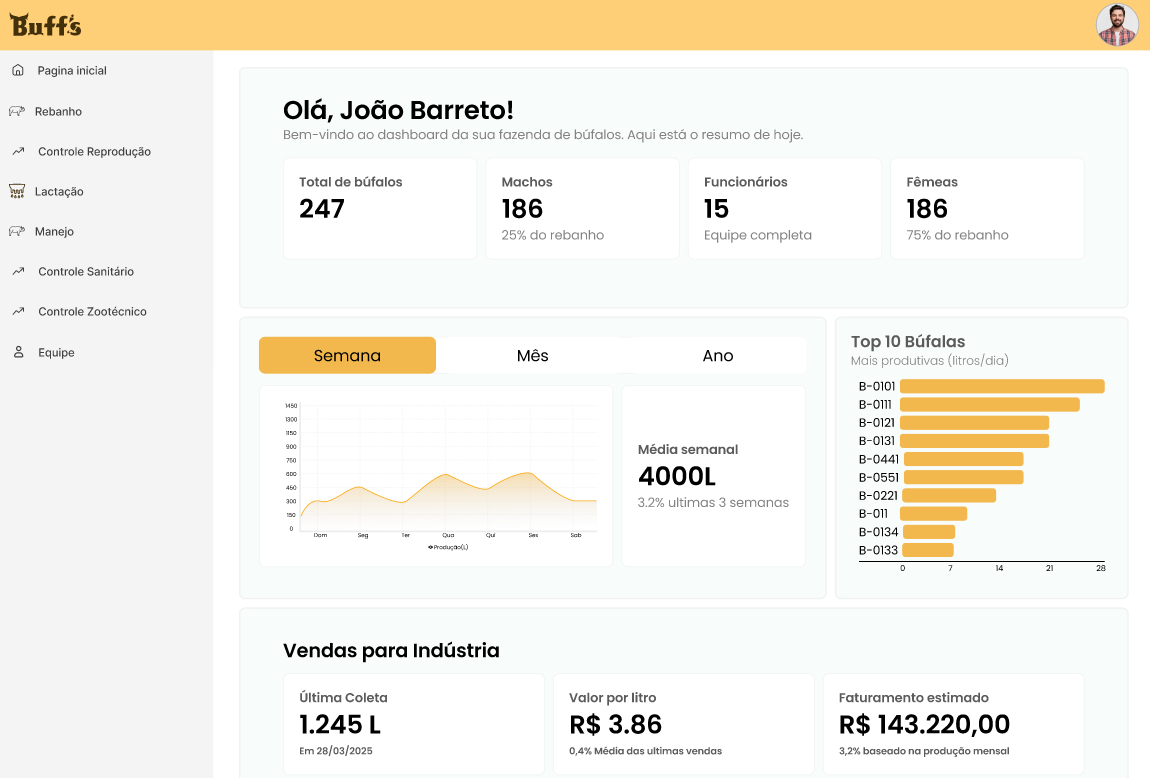
\includegraphics[scale=0.3]{fig1a.png}
\SourceOrNote{Autoria Própria (2024)}
\end{figure}

A primeira seção, ilustrada na Figura \Cref{fig:02}, é a de Gestão de Rebanho, onde é possível visualizar todos os bubalinos que compõem o rebanho, distribuídos por maturidade (bezerros, novilhas, vacas e touros), sexo e raça, com a contagem total de cada categoria.

\begin{figure}[!h]
\centering
\caption{Aplicação WEB - Gestão do Rebanho}%
\label{fig:02}
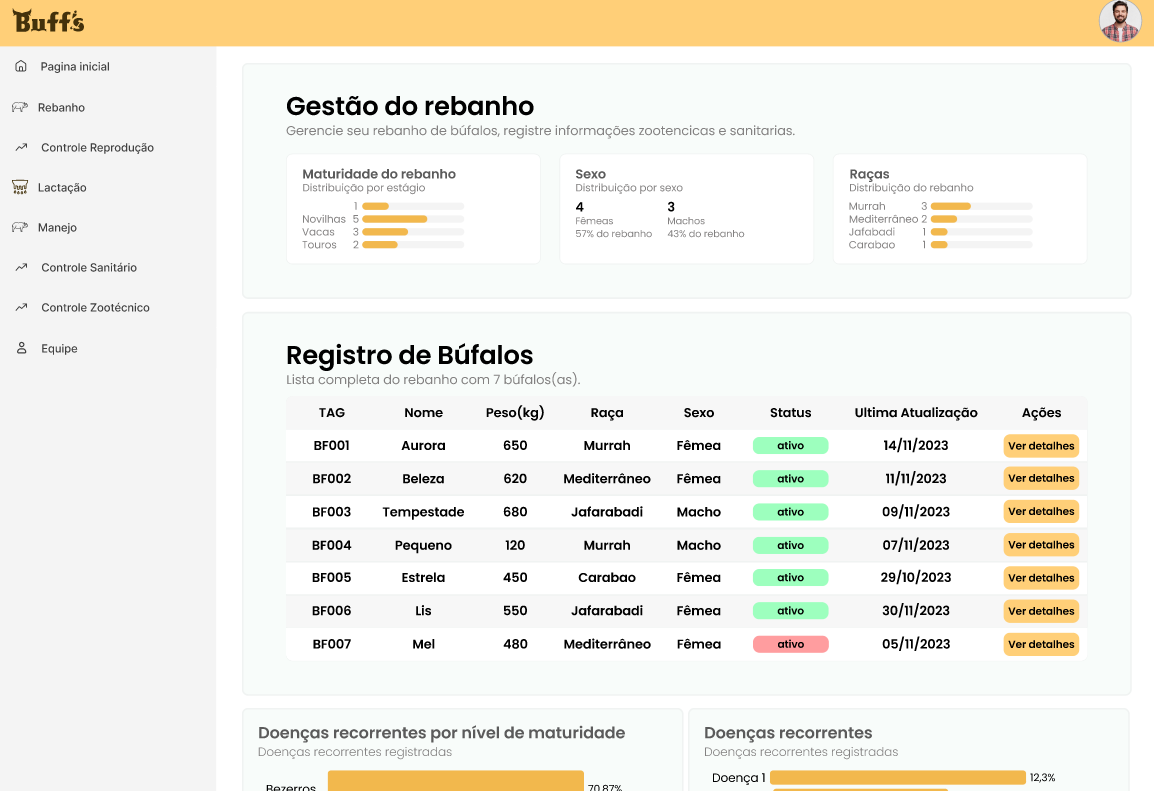
\includegraphics[scale=0.3]{fig1b.png}
\SourceOrNote{Autoria Própria (2024)}
\end{figure}

Na seção de Lactação, mostrada na Figura \Cref{fig:03}, o usuário pode acompanhar a quantidade de leite produzida diariamente, semanalmente, mensalmente e anualmente, desde que os dados sejam devidamente alimentados na plataforma. Além disso, é possível comparar os rendimentos por períodos, por meio de gráficos que facilitam o entendimento visual das informações. A plataforma também destaca as búfalas que não estão produzindo, sinalizando um possível atraso ou problema no manejo da fazenda.

\begin{figure}[!h]
\centering
\caption{Aplicação WEB - Gestão Lactação}%
\label{fig:03}
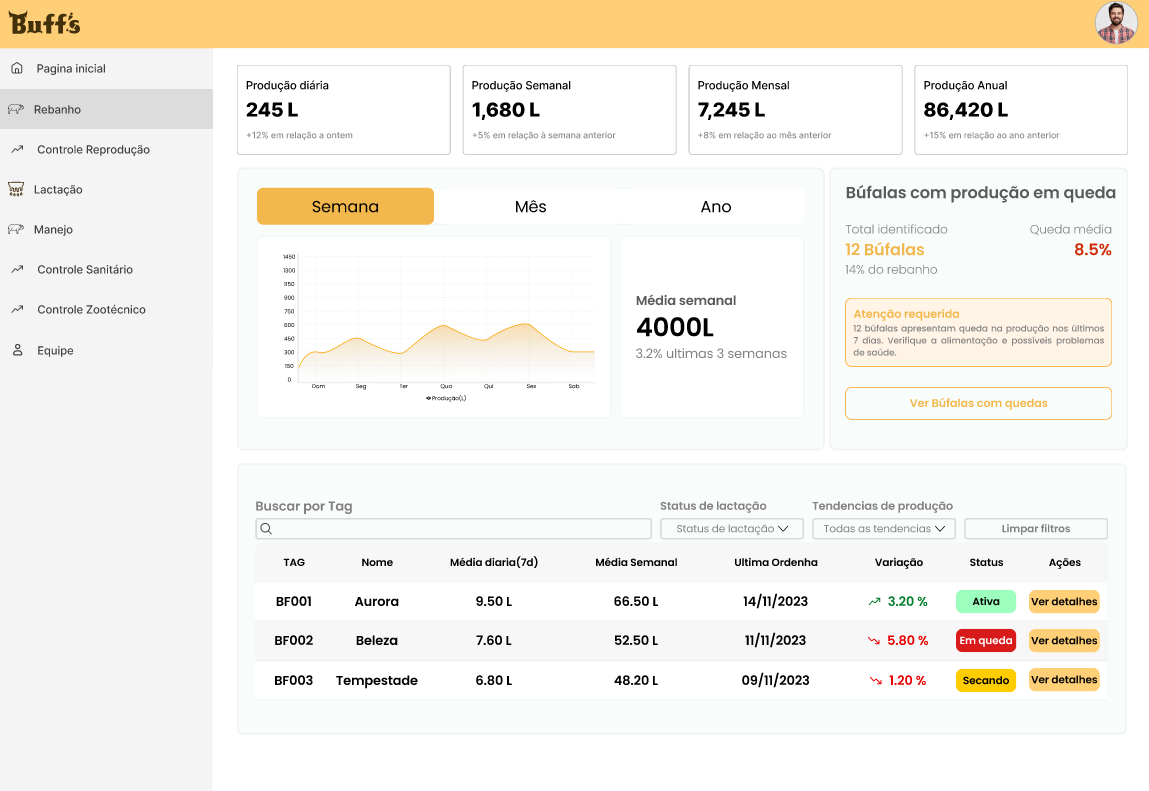
\includegraphics[scale=0.3]{fig1c.png}
\SourceOrNote{Autoria Própria (2024)}
\end{figure}

\subsection{METODOLOGIA DE DESENVOLVIMENTO DA REDE} 

O sistema de estrutura de rede da aplicação é composto por três partes principais: o Front-end, acessado tanto por dispositivos móveis quanto por navegadores em desktops; uma API desenvolvida em Node.js, responsável por centralizar toda a comunicação entre o Front-end e a base de dados; e a base de dados, onde todas as informações persistentes são armazenadas.

O fluxo de comunicação inicia-se a partir de uma interação do usuário com a interface da aplicação, que envia uma requisição para a API. Esta, por sua vez, interpreta a solicitação e realiza uma das quatro operações previstas no modelo CRUD, sigla para Create, Read, Update e Delete, representando, respectivamente, as ações de criar, consultar, atualizar e excluir dados no banco.

Cada requisição é processada de acordo com a operação correspondente. Quando o usuário insere novos dados, a API executa a operação de criação (Create); ao consultar informações, realiza uma leitura (Read); quando edita registros, processa uma atualização (Update); e ao excluir, executa uma operação de exclusão (Delete). No entanto, por boas práticas de segurança e controle de histórico, o sistema não realiza a exclusão física dos dados. Em vez disso, os registros são marcados como inativos, mantendo-se disponíveis na base para futuras consultas, auditorias ou reativações, caso necessário.

\begin{flowchart}[!htb]
\centering
\caption{Arquitetura do Fluxo das redes}%
\label{fcht:ex-algorithm}
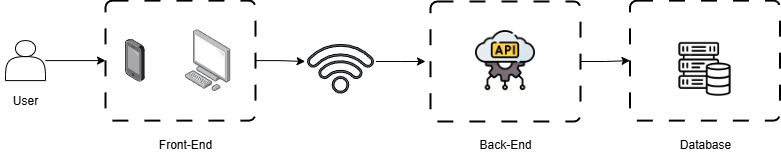
\includegraphics[scale=0.4]{arquiteturaDoFluxo}
\SourceOrNote{Autoria Própria (2024)}
\end{flowchart}